\section{Introduction}


Scaling test-time compute in large language models (LLMs) helps improve the performance across a wide range of tasks including reasoning, coding~\citep{DBLP:conf/iclr/WuSLWY25,DBLP:journals/corr/abs-2408-03314, DBLP:journals/corr/abs-2501-19393, DBLP:journals/corr/abs-2501-19306}. 
Mainstream scaling strategies such as sequential~\citep{DBLP:conf/nips/MadaanTGHGW0DPY23} and parallel scaling~\citep{DBLP:conf/iclr/0002WSLCNCZ23,DBLP:journals/corr/abs-2407-21787} enable models to utilize more effort, elicit deeper reflection, and refine their outputs, often leading to substantial gains in answer quality~\citep{DBLP:journals/corr/abs-2503-24235}. These successes motivate recent efforts to extend test-time scaling to tool-augmented agents~\citep{DBLP:journals/corr/abs-2506-12928, DBLP:journals/corr/abs-2508-00890}, where LLMs are equipped with various tools to interact with the external environment such as search engines or APIs.



Test-time scaling for tool-augmented agents expands both thinking (tokens) and acting (tool calls). While textual reasoning tasks are usually scaled by thinking with more tokens, solely increasing the internal thinking effort in agents proves to be suboptimal and does not always translate to performance scaling~\citep{DBLP:journals/corr/abs-2506-07976}.
Unlike controlling the token count in textual reasoning~\citep{DBLP:conf/acl/HanWFZM025,DBLP:journals/corr/abs-2504-13367}, in agent tasks such as web browsing, the number of tool calls directly determines the depth and breadth of exploration~\citep{anthropic2025context, miromindteam2025mirothinkerpushingperformanceboundaries}, defining the effective boundary of external information access.





However, simply granting agents more test-time tool-call resources does not guarantee better performance. Our analysis reveals a critical bottleneck: \emph{standard agents lack inherent budget awareness}. Without explicit signals, they often perform shallow searches~\citep{lu2025deepdiveadvancingdeepsearch} and fail to utilize additional resources, even when available. As our empirical findings later demonstrate, standard agents quickly hit a ``performance ceiling'', saturating their capabilities regardless of how much extra budget is allocated.
The challenge is not simply spending more, but spending wisely: the marginal benefit per tool call is uncertain, so every call must be spent strategically.


\begin{figure}[t!] 
    \centering
    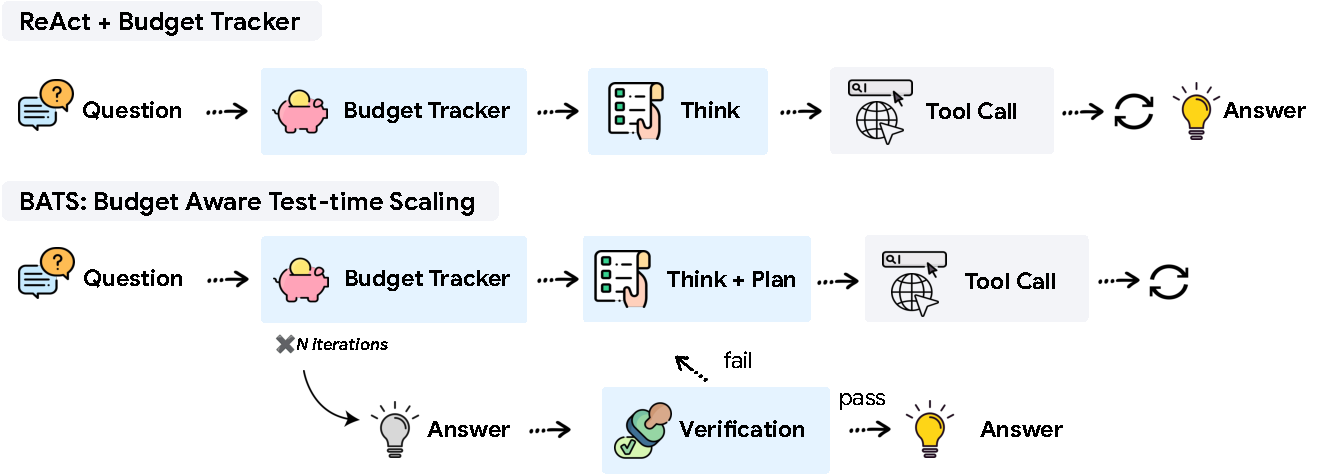
\includegraphics[width=0.8\textwidth]{assets/figs/bt_bats.pdf} 
    \caption{Budget Tracker is a lightweight plug-in that can be applied to both a standard ReAct agent (top) and more advanced orchestration frameworks like BATS (bottom). In this figure, blue boxes highlight modules that adapt to the budget.}
    \label{fig:bt_bats}
\end{figure}


This unique complexity brings up a critical research question: How can tool-augmented agents scale \emph{effectively} by making the best use of a given resource budget?
We study this question in a budget-constrained setting, grounding our analysis in search agents equipped with search and browse tools, which are widely used in practice~\citep{google2025geminideepresearch, openai2025deepresearch} and inherently require extensive tool calls to collect external information.
To ensure a fair and transparent comparison, we formalize a unified cost metric that jointly accounts for the economic costs of both internal token consumption and external tool interactions. This metric enables us to trace a true cost-performance scaling trend.



We first develop an intuitive, light-weight approach: \textbf{Budget Tracker} (Figure~\ref{fig:bt_bats} (top)), which is a plug-and-play module compatible with most ReAct-based agents~\citep{DBLP:conf/iclr/YaoZYDSN023}. Budget Tracker provides the agent with a continuous signal of resource availability, proving to be a simple yet effective method for enabling budget-aware tool use. Through extensive experiments, we show that this simple plug-in improves performance across various budget constraints. Combining this explicit budget awareness with traditional test-time scaling strategies consistently enables more effective scaling behaviors while continuously pushing the cost-performance Pareto frontier.



While simple awareness is effective, it still operates within the agent's predefined logic. To further break the scaling ceiling and fully internalize resource constraints, we introduce \textbf{\method} (\textbf{B}udget \textbf{A}ware \textbf{T}est-time \textbf{S}caling) (Figure~\ref{fig:bt_bats} (bottom)), a framework designed to maximize agent performance under any given budget. At its core, \method maintains a continuous signal of remaining resources, and it uses this information to dynamically adapt its behavior. A planning module adjusts stepwise effort to match the current budget, while a verification module decides whether to ``dig deeper'' into a promising lead or ``pivot'' to alternative paths based on resource availability.


Our empirical study systematically evaluates the relationship between overall resource cost and task performance by comparing different scaling frameworks under varying budgets.
The results show that \method produces more favorable scaling curves: it achieves higher performance while using fewer tool calls and incurring lower overall cost than competing methods.
These findings demonstrate the potential of budget-aware design for creating effective and efficient tool-augmented agents, highlighting the importance of explicitly accounting for cost in agent test-time scaling.


We summarize our contributions as follows:
\begin{itemize}
    \item We provide the first systematic study of budget-constrained tool-use agents by formalizing agent test-time scaling with explicit tool-call budgets and introducing a unified cost metric.
    \item We introduce \textbf{Budget Tracker}, a light-weight, plug-in module compatible with any agent orchestration framework that enables effective budget-aware tool use.
    \item We develop \textbf{\method}, a budget-aware framework that dynamically adapts planning and verification strategies based on real-time resource tracking, flexibly switching between deepening a lead and branching to alternatives.
    \item We conduct systematic experiments under varying budgets and unified costs with search agents, demonstrating that \method is more cost-effective and yields more favorable scaling curves and better cost–performance trade-offs. 
\end{itemize}
